% SPDX-FileCopyrightText: 2026 Hasan Melih Akbulut
% SPDX-License-Identifier: CC-BY-4.0

\chapter{Physical design}
\label{ch:phys}

The layout is the run \code{s83romecc5}, completed 2026-09-13: the
eight-macro build, carrying the two check macros that hold the boot
ROM's error-correcting code (\dcite{67}{section 11}), and a layout that
meets hold at all three corners. Its own
\code{final/metrics.json} is the source for every unattributed number
below; a figure from a superseded layout is marked with its date, the
rule \dcite{64}{} sets.

\textbf{No clock frequency is claimed for this design.} The flow is
given a \qty{20}{\nano\second} period as a constraint, and every timing
result here is a slack against it at a named corner. An early layout
document derived a frequency from its own worst slack;
\dcite{53}{section 9.2} refused to publish that figure or any other, on
three grounds --- it is a number a run reached rather than a
requirement, it is a measured non-closure, and the project's other part
carries a different declared clock --- and every physical document since
reports slack against \qty{20}{\nano\second} and nothing else.

\section{The flow, and what is pinned}

The chain is rootless: no container, no system package, no root. Each
binary is fronted by a shim that establishes only its own
\code{LD\_LIBRARY\_PATH}, because the OpenROAD build ships a newer glibc
that segfaults every other host binary if it leaks into the ambient
environment (\dcite{12}{section 2.1}). \Cref{tab:phys-tools} is the pin
list~\cite{lamb2022}.

\begin{table}[tbp]
\centering
\caption{The pinned toolchain (\dcite{12}{section 2.2}, recorded
2026-08-25 in this environment). The PDK commit~\cite{ihppdk} is not
chosen: every LibreLane~\cite{openlane2020} release ships
\code{pdk\_hashes.yaml} naming the commit it was tested against, and the
runner reads that pin out of the installed wheel and refuses to run
against anything else.}
\label{tab:phys-tools}
\small
\begin{tabular}{@{}ll@{}}
\toprule
\textbf{Component} & \textbf{Version} \\
\midrule
LibreLane & v3.0.5 \\
Ciel (PDK manager) & v2.6.1 \\
Python & 3.12.3 \\
OpenROAD & 26Q1-2938-g0e2d771c5e \\
Yosys & 0.67 (2d1509d1b) \\
KLayout & 0.30.9 \\
Magic & 8.3.678 \\
Netgen & 1.5.272 \\
IHP-Open-PDK & \code{c4b8b4e5e7a05f375cca3815d51b3a37721fbf5c} \\
Standard cells & \code{sg13g2\_stdcell}, 84 Liberty cells \\
\bottomrule
\end{tabular}
\end{table}

\textbf{The flow does not synthesise, and that is a decision.} The
runner hands LibreLane a netlist as an initial state and skips
\code{Yosys.Synthesis}, because both hierarchy modes are wrong for this
design in opposite directions. Under \code{flatten}, Yosys honours the
\code{keep\_hierarchy} attribute the triple-modular register bank carries
as an anti-merge defence~\cite{esa_ftmr} and
\code{Checker.\allowbreak YosysUnmappedCells} stops the run; under
\code{deferred\_flatten}, a constant driving the core's
\code{cheriot\_enable\_i} never folds, and the same RTL comes out as
37,895 cells of \qty{523809.6444}{\micro\metre\squared} against 27,565 of
\qty{396177.6420}{\micro\metre\squared}, and its worst slow-corner path is
\qty{13.8442}{\nano\second} worse, measured before any placement exists
at all (\dcite{47}{sections 6.2 and 6.3}). The project's own script holds
\code{keep\_hierarchy} through optimisation and \code{abc} and releases
it before the final flatten.

\textbf{The flow is deterministic, and that is measured.} Two runs of
the same netlist give metrics files with 199 keys and zero differing,
and byte-identical DEF, ODB, netlist, SDC, LEF, Liberty and SPICE. The
only seed anywhere in it is \code{detailed\_route -or\_seed 42},
hard-coded in LibreLane's \code{drt.tcl}, and resuming the router at ten
threads instead of this machine's twenty gives a byte-identical database
(\dcite{71}{sections 3, 5 and 8}). \emph{Every difference between two
layouts here is therefore a difference the netlists caused.}

\section{The floorplan}

\begin{figure}[tbp]
  \centering
  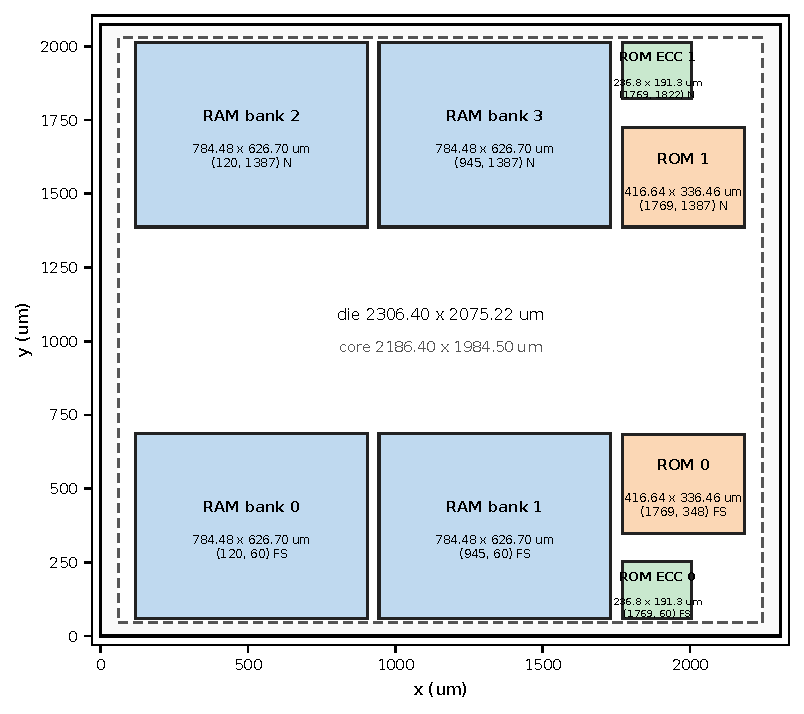
\includegraphics[width=\linewidth]{figures/floorplan_macros.pdf}
  \caption[The floorplan and the eight macros]{The die outline, the core
  area and the eight vendor macros with their sizes, origins and
  orientations, drawn from the sign-off run's own DEF by
  \code{thesis/figures/\allowbreak make\_layout\_figures.py}. Two macro
  rows face a \qty{700.08}{\micro\metre} standard-cell channel; the
  third column carries the boot ROM and, in the height the shorter ROM
  macro leaves over in each row, its two check macros. These eight are
  the only instances on the die whose position a person chose.}
  \label{fig:phys-floorplan}
\end{figure}

The die is $2306.40 \times 2075.22$\,\si{\micro\metre}, reported as
\qty{4786290}{\micro\metre\squared} and exactly
\qty{4786287.408}{\micro\metre\squared} as the product of the DEF's own
\code{DIEAREA} corners (\dcite{59}{section 4.1}). The core runs from
$(60.00,\,45.36)$ to $(2246.40,\,2029.86)$\,\si{\micro\metre}:
$2186.40 \times 1984.50$\,\si{\micro\metre} and
\qty{4338910}{\micro\metre\squared}. Alignment is asserted rather than
arranged --- \num{2186.40} is exactly 4,555 sites of
\qty{0.48}{\micro\metre} and \num{1984.50} exactly 525 rows of
\qty{3.78}{\micro\metre}, and every macro origin is an integer number of
sites and rows from the core's lower left corner
(\dcite{47}{section 6.1}) --- and \code{hw/soc/pnr/floorplan.py} refuses
to emit a floorplan that has lost the property, reading macro
dimensions from the installed PDK's LEF rather than from a transcript.

\begin{table}[tbp]
\centering
\caption{The eight macros, from the run's own \code{resolved.json} and
the vendor LEF \code{SIZE} statements. All eight are \code{FIXED}.}
\label{tab:phys-macros}
\small
\begin{tabular}{@{}llrrl@{}}
\toprule
\textbf{Instance} & \textbf{Master} & \textbf{$W \times H$, \si{\micro\metre}} & \textbf{Origin, \si{\micro\metre}} & \textbf{Orient} \\
\midrule
\code{u\_ram...u\_b0} & \code{2048x64} & $784.48 \times 626.70$ & (120.00,\,60.48) & FS \\
\code{u\_ram...u\_b1} & \code{2048x64} & $784.48 \times 626.70$ & (944.64,\,60.48) & FS \\
\code{u\_ram...u\_b2} & \code{2048x64} & $784.48 \times 626.70$ & (120.00,\,1387.26) & N \\
\code{u\_ram...u\_b3} & \code{2048x64} & $784.48 \times 626.70$ & (944.64,\,1387.26) & N \\
\code{u\_rom...u\_b0} & \code{1024x32} & $416.64 \times 336.46$ & (1769.28,\,347.76) & FS \\
\code{u\_rom...u\_b1} & \code{1024x32} & $416.64 \times 336.46$ & (1769.28,\,1387.26) & N \\
\code{u\_rom...u\_c0} & \code{512x16} & $236.80 \times 191.34$ & (1769.28,\,60.48) & FS \\
\code{u\_rom...u\_c1} & \code{512x16} & $236.80 \times 191.34$ & (1769.28,\,1821.96) & N \\
\bottomrule
\end{tabular}
\end{table}

\Cref{fig:phys-floorplan} and \cref{tab:phys-macros} are the
arrangement, and \textbf{it is forced rather than chosen: the forcing
constraint is pin geometry.} Every \code{RM\_IHPSG13} part puts all of
its signal pins on one edge, at local $y=0$, on Metal2 and Metal3 ---
352 on the $2048\times64$ and 190 on the $1024\times32$
(\dcite{47}{section 6.1}) --- and a macro whose pin edge faces another
macro is a macro the router reaches the long way round. The lower row is
therefore \code{FS}, which mirrors about $X$ and lifts its pins to its
\emph{top}; the upper row is \code{N}, which leaves its pins at its
\emph{bottom}; and both face the \qty{700.08}{\micro\metre} channel
between them. Rotating a hard macro is not an option this project can
check, for the reason \cref{sec:phys-decks} gives.

\textbf{The two ROM check macros fit without growing the die, and why
they sat unplaced for weeks is worth more than the placement.} The open
item read that there was \qty{60.48}{\micro\metre} beside each ROM and
the check part is \num{236.80} wide --- true, and a measurement of the
wrong axis. A macro row is as tall as the RAM,
\qty{626.70}{\micro\metre}; the ROM is \num{336.46}; the third column
therefore carries \qty{290.24}{\micro\metre} of unused height per row
and the check macro is \num{191.34} tall. The real obstacle was pins:
the bottom row is \code{FS}, so its ROM's pins are at its top and a
check macro in the pocket \emph{above} it would sit across every wire
leaving them. The bottom ROM is raised to the top of its own band, to
$y=347.76$, and the check macro takes the blind space beneath;
clearances are \qty{95.94}{\micro\metre} and \qty{98.24}{\micro\metre}
with a \qty{10}{\micro\metre} halo, computed from the LEF size and row
pitch and asserted, never written down as a coordinate
(\dcite{67}{section 11}). The die, the core and the four RAM origins do
not move, which keeps measurements on the earlier six-macro floorplan
comparable with these.

\textbf{The die has named zones, and they are the vocabulary the rest of
this chapter uses}, as \code{hw/soc/pnr/\allowbreak clint\_region.py}
defines them after \dcite{72}{section 6.4}: the \emph{channel} is
$687.18 \le y < 1387.26$; the \emph{upper} and \emph{lower pockets} are
the areas at $x \ge 1769.28$ above each ROM, each including the strip
beside it at that height; the \emph{strip} is $x \ge 2185.92$. One
caveat comes with the definition, because the figures inherit it: those
constants are the six-macro floorplan's, in which the lower ROM sat at
$y=60.48$. Here it is at \num{347.76} with the check macro beneath, so
the zone predicate and the ``lower pocket'' outline in
\cref{fig:phys-density} describe the earlier geometry, and the zone
census quoted below is a measurement on that earlier layout.

\textbf{Forced is not untested.} Two alternatives were hardened --- a
channel of 82 rows instead of 185, and a die \qty{19.8}{\percent}
narrower with the ROMs as islands --- and both are worse at every stage
measured, by \qty{0.84}{\nano\second} and \qty{1.70}{\nano\second} at
post-clock-tree and, for the one that routes, \qty{10.09}{\nano\second}
after global routing on \qty{44.1}{\percent} more wirelength. Shrinking
the die spread the logic rather than compacting it: the tight variant
exiled 7,857 of 27,558 cells into the ROM pockets against 739
(\dcite{48}{sections 4 and 5}).

\section{Where the logic went}

\begin{figure}[tbp]
  \centering
  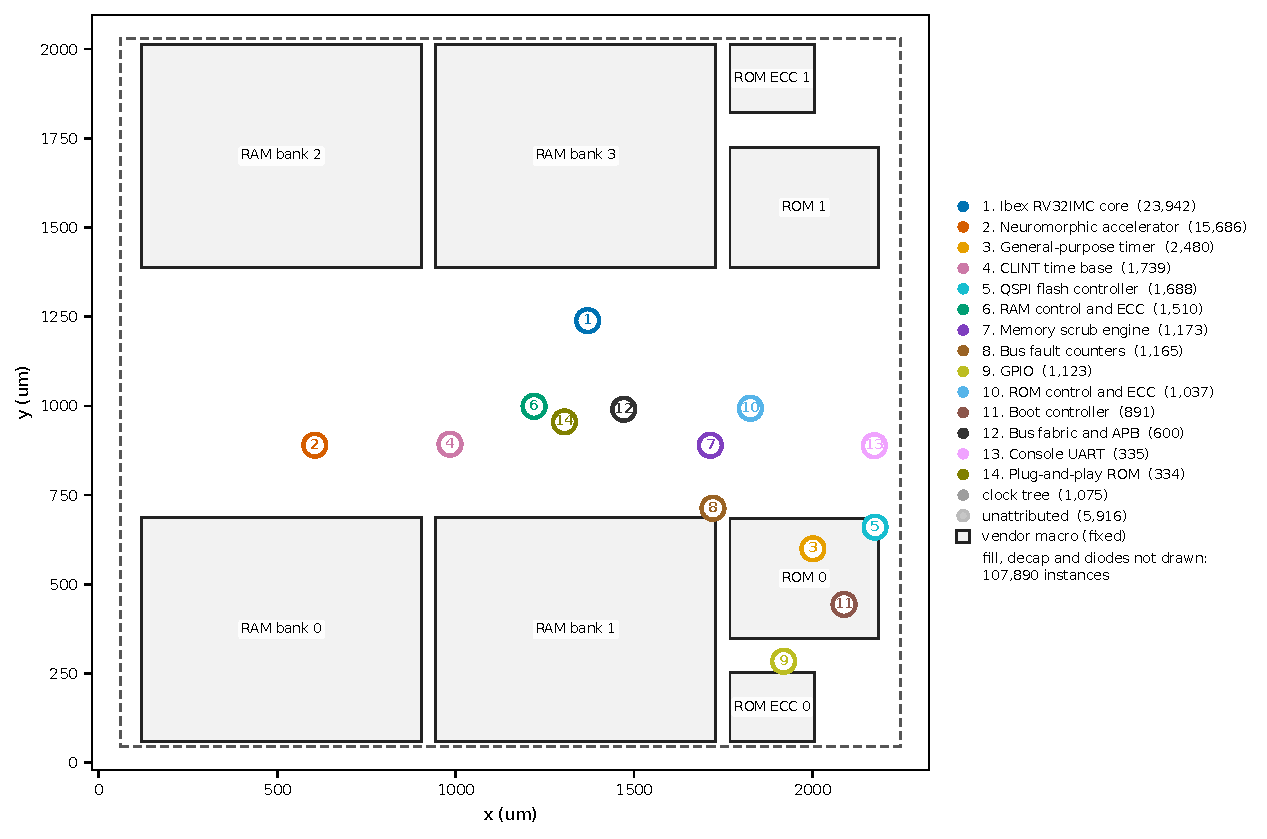
\includegraphics[width=\linewidth]{figures/layout_blocks.pdf}
  \caption[The whole die, coloured by block]{Every standard cell in the
  sign-off layout, coloured by the block it was attributed to, with the
  macros drawn, a numbered centroid per block and per-block counts in
  the legend; the 107,890 fill, decap and diode instances are not drawn.
  Apart from the macros, nothing here was told where to go. The
  attribution method and its \qty{9.75}{\percent} unresolved remainder
  are described in the text; a centroid is a mean and can land on a
  macro, which is why markers 3 and 11 sit inside ROM~0.}
  \label{fig:phys-blocks}
\end{figure}

\Cref{fig:phys-blocks} answers ``where is the processor, where is the
memory'' for a die carrying 168,592 instances, and it must be read with
its method in hand.

\textbf{Exactly one cell on this die could be coloured by its own name.}
Synthesis runs \code{synth -flatten} and then \code{abc}, so of the
168,592 instance names in the DEF only 1,140 carry a dot and 632 of
those are the RAM's; colouring only those would colour a few per cent of
the die and put the processor in the wrong place, because the register
file keeps its name and the arithmetic unit does not. Attribution is
therefore by connectivity, in three passes: Yosys keeps the hierarchical
name of any net it did not create, so every net named after a top-level
instance votes for that block; each anonymous cell takes the block most
of its pins' nets vote for; and cells still unattributed take the
majority block of the cells they share a net with, twice. Clock buffers,
ties, fill and decap are recognised by name or master and form their own
classes (\code{thesis/figures/\allowbreak make\_layout\_figures.py}).

\textbf{The error bar is printed rather than hidden, and it is larger
than the headline figure suggests.} Of the 60,694 non-fill instances,
\code{thesis/figures/\allowbreak layout\_attribution.json} records 1
attributed by its own name, 643 named nets producing 19,790
attributions by vote, 1,075 classified as clock tree, and 5,916 ---
\qty{9.75}{\percent} --- never resolved, drawn grey and counted in the
legend. The remaining 33,912, \qty{55.9}{\percent} of the non-fill
instances, came from the two rounds of neighbour propagation (arithmetic
on that file's own fields). These maps show where the placer put each
block's logic with most of the attribution from the weakest of the three
passes; the per-block counts are an attribution with that error bar on
them, not a census.

\begin{figure}[tbp]
  \centering
  
\includegraphics[width=\linewidth]{figures/layout_panels.pdf}
  \caption[One panel per block]{The nine most populous blocks, each
  against the whole die in grey. The core fills the upper channel and
  reaches into the upper pocket; the accelerator fills the lower channel
  and the left margin; the peripherals cluster at the right, beside and
  below the ROM macros; the RAM's control and error-correcting logic is
  a thin band on both macro rows' pin edges.}
  \label{fig:layout_panels}
\end{figure}

\Cref{fig:layout_panels} separates what \cref{fig:phys-blocks}
interleaves. The core's 23,942 attributed instances take the upper half
of the channel; the accelerator's 15,686 take the lower half and the
left margin. The RAM control and ECC block's 1,510 instances are not a
blob but a thin band along the facing edges of both macro rows --- it is
the logic that fans out to four macros' pins, and the placer put it on
the pins. The CLINT's 1,739 are the tightest cluster on the die, one
compact blob mid-channel, which matters in \cref{sec:phys-clint};
everything with an external interface sits in the third column, in the
pockets and the strip beside the ROMs, about as far from the RAM as the
core box allows.

\begin{table}[tbp]
\centering
\caption{The instance census, from the run's own
\code{final/metrics.json}. Instance utilisation counts standard cells
and macros against the core area; standard-cell utilisation counts
standard cells against the core area less the macros.}
\label{tab:phys-census}
\small
\begin{tabular}{@{}lr@{}}
\toprule
\textbf{Quantity} & \textbf{Value} \\
\midrule
Instances, total & 168{,}592 \\
\quad vendor macros & 8 \\
\quad standard cells, excluding fill & 64{,}349 \\
\quad fill cells & 104{,}235 \\
\quad antenna cells (of which diodes) & 1{,}575 (1{,}258) \\
Sequential cells & 5{,}998 \\
Integrated clock-gating cells & 3 \\
Timing-repair buffers & 13{,}089 \\
\quad inserted for setup / for hold & 369 / 11 \\
Clock buffers / clock inverters & 815 / 309 \\
Standard-cell area, \si{\micro\metre\squared} & 933{,}010 \\
Macro area, \si{\micro\metre\squared} & 2{,}337{,}520 \\
Rows / sites & 1{,}517 / 1{,}003{,}595 \\
Instance utilisation & 0.7538 \\
Standard-cell utilisation & 0.4662 \\
Legalisation displacement, mean / max, \si{\micro\metre} & 0.075 / 20.04 \\
\bottomrule
\end{tabular}
\end{table}

\Cref{tab:phys-census} is the census. The macros are
\qty{48.8}{\percent} of the die area, and the placeable area left inside
the core --- the core less the macros, which is the denominator the
flow's own utilisation metric uses --- is
\qty{2001390}{\micro\metre\squared}, of which the standard cells fill
\qty{46.6}{\percent}. That denominator is generous: on the six-macro
floorplan \dcite{59}{section 11} measured the union of the DEF's
\code{ROW} statements at \qty{7.66}{\percent} less than it, the macro
halos and the site grid taking the difference. The first layout of this
SoC put \qty{396177.6420}{\micro\metre\squared} of cells into
\qty{2092010.95}{\micro\metre\squared} (\dcite{48}{section 4.1}),
\qty{18.9}{\percent}, and
\dcite{47}{section 8.4} named that sparseness as the probable cause of
what layout was costing in timing. It was not: what has since filled the
die is the design.

\begin{figure}[tbp]
  \centering
  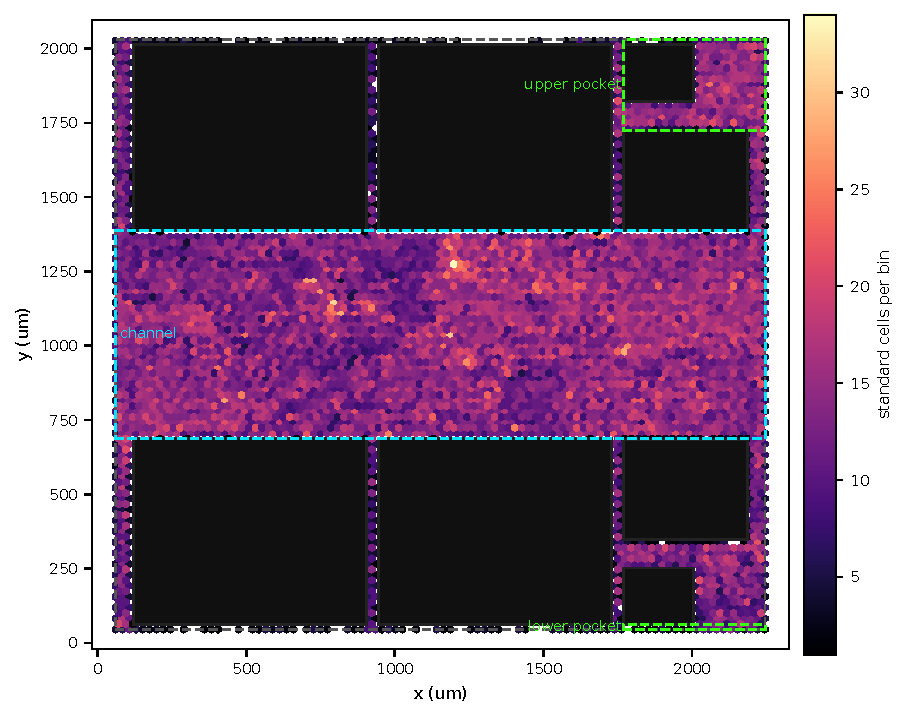
\includegraphics[width=\linewidth]{figures/layout_density.pdf}
  \caption[Standard-cell density over the core]{Hexbin density of the
  non-fill standard cells, macros in black, channel and pocket zones
  outlined. The channel is populated almost uniformly and the rest of
  the logic is in the pockets and the strip at the right. The ``lower
  pocket'' rectangle is drawn from the six-macro floorplan's constants,
  in which the lower ROM sat at $y=60.48$; in this layout the check
  macro stands there, so that outline no longer marks a pocket.}
  \label{fig:phys-density}
\end{figure}

\Cref{fig:phys-density} is the same placement as a density field, and
what it shows is where the logic went: \emph{the channel is not where
all of it is}. That is not what the timing turns on, and the difference
was measured rather than assumed --- on this same run, wire is
\qty{1.9}{\percent} of a violating path at the median and
\qty{3.0}{\percent} at the most wire-bound of 1{,}000, over a median of
78 gate stages, and the CLINT closure the pocket story was about sits
1{,}802 cells of 1{,}802 in the channel with none in either pocket
(\dcite{83}{sections 1, 2 and 3}). The zone census on the six-macro floorplan puts
45,619 standard cells in the channel, 2,222 in the upper pocket, 3,568
in the lower pocket, 441 in the strip and 436 elsewhere, against a
baseline run of the same floorplan at 45,966 / 2,208 / 3,049 / 424 /
173. Those runs differ by 466 cells of netlist, and the extra cells did
not go into the channel --- it holds 347 \emph{fewer}, and the pockets,
the strip and everything outside them 813 more. A net with one pin in
the upper pocket and one in the channel crosses a ROM macro, and 140
nets did so in one run and 134 in the other (\dcite{72}{section 6.4}).

\section{Timing}
\label{sec:phys-timing}

The flow analyses three corners. It names them exactly, and so does
this chapter: \code{nom\_slow\_\allowbreak 1p08V\_125C},
\code{nom\_typ\_\allowbreak 1p20V\_25C} and
\code{nom\_fast\_\allowbreak 1p32V\_m40C}. Sign-off timing is on
extracted parasitics, at a \qty{20}{\nano\second} period, with a
\qty{5}{\percent} derate, \qty{0.25}{\nano\second} of clock uncertainty
and clock-reconvergence pessimism removal. \code{PNR\_CORNERS} is the
typical and slow pair, so the fast corner is not \emph{optimised}
against during the flow --- but all four corner checkers see all three,
which is what \cref{tab:phys-timing} depends on.

\begin{table}[tbp]
\centering
\caption{Sign-off timing of \code{s83romecc5}: three corners, extracted
parasitics, \qty{20}{\nano\second} period (the run's step-49
\code{summary.rpt} and its \code{final/metrics.json}). No frequency is
derived from any of it.}
\label{tab:phys-timing}
\small
\begin{tabular}{@{}lrrrrrr@{}}
\toprule
\textbf{Corner} & \textbf{Setup WS} & \textbf{Vio} & \textbf{Setup TNS} & \textbf{Hold WS} & \textbf{Vio} & \textbf{Slew} \\
 & ns & & ns & ns & & vio \\
\midrule
\code{nom\_slow\_1p08V\_125C} & $-7.5758$ & 3{,}529 & $-14{,}735.65$ & $+0.4261$ & 0 & 533 \\
\code{nom\_typ\_1p20V\_25C}   & $+2.6396$ & 0 & 0 & $+0.1769$ & 0 & 77 \\
\code{nom\_fast\_1p32V\_m40C} & $+8.3630$ & 0 & 0 & $+0.0296$ & 0 & 20 \\
\bottomrule
\end{tabular}
\end{table}

\textbf{Hold is met at all three corners; setup misses at the slow
corner by \qty{7.5758}{\nano\second} on 3,529 endpoints.} There are also
533 max-slew violations at the slow corner and 98 max-cap violations at
the fast, and the flow exits non-zero naming them --- which it does only
because four keys were set before the first run rather than audited
after it (\dcite{47}{section 7}). Shipped,
\code{SETUP\_VIOLATION\_\allowbreak CORNERS} falls through to the PDK's
\code{["*typ*"]}, so setup would have been examined at the typical
corner alone, where this design passes; and the max-cap and max-slew
checkers' step classes override their corner lists to \code{[""]}, which
is truthy, so the list filters to empty, no corner matches, and the step
\emph{warns} instead of failing. All four are \code{["*"]} here. A fifth
key is a type rather than a value: the derate ships as the integer
\num{5} and \code{base.sdc} computes \code{expr 5 / 100} in Tcl, which
is \num{0}, so nothing is derated while the log says otherwise; the
configuration sets \num{5.0}, and \code{resolved.json} cannot audit it
because it flattens the float back --- a trap that has now bitten in
four places (\dcite{72}{section 7.1}).

Two metrics the flow judges with nothing are reported here rather than
left in a file. \code{Checker.\allowbreak WireLength} has no threshold
in either PDK and so warns and skips, on a layout whose longest routed
net is \qty{4292.89}{\micro\metre}. And the Classic flow has no
max-fanout checker at all, on a layout carrying 589 such violations
against a constraint of 10 and a library declaring
\code{default\_max\_fanout : 8}.

\subsection{The worst path}

\code{hw/soc/pnr/\allowbreak violator\_census.py} resolves all 3,529
violating endpoints against the run's own netlist and finds six launch
points behind them. One is the register file's read address bit
\code{raddr\_b\_i[4]}, which launches 2,865 of them and carries
\qty{-13195.08}{\nano\second} of total negative slack. The others are
360 endpoints from a RAM macro's \code{A\_DOUT[31]}, 154 from
\code{raddr\_b\_i[2]}, 101 from the accelerator's axon register, 38 from
a launch point the census cannot resolve to a public name, and 11 from
the CLINT's \code{mtime} codeword register.

The worst is \emph{a register-file read address into the register file's
own error-correcting encoder}, ending at the check bit
\code{g\_rf\_flops[2].\allowbreak g\_chk.rf\_chk\_q[6]} of that file's
single-error-correcting double-error-detecting code. It decomposes into \qty{2.492291}{\nano\second} of launch clock ---
through the core's integrated clock gate, which is in the launch path
--- and a data path of \qty{27.0731}{\nano\second} over \textbf{77
driver stages, of which \qty{26.290}{\nano\second} is cell delay and
\qty{0.7827}{\nano\second} is net delay}, arriving at
\qty{29.565346}{\nano\second} against a required
\qty{21.989546}{\nano\second}, for \qty{-7.575801}{\nano\second} of
slack (step-49 \code{max.rpt}, slow corner). Seventeen of the 77 stages
are \code{sg13g2\_xnor2\_1}, which is the encoder; eighteen are buffers
or inverters, and fifteen of those carry the \code{rebuffer} or
\code{fanout} names the repair steps give what they insert.

\textbf{Two stages cost \qty{5.701}{\nano\second} between them, and why
neither was repaired is a property of the library rather than of the
resizer.} One \code{sg13g2\_nand4\_1} drives \qty{216.9}{\femto\farad}
to a single load for \qty{3.034}{\nano\second} at a
\qty{3.839}{\nano\second} transition; one \code{sg13g2\_xnor2\_1} drives
\qty{283.6}{\femto\farad} for \qty{2.667}{\nano\second} at
\qty{3.627}{\nano\second}. Both loads are \emph{legal}: the slow-corner
Liberty declares \code{default\_max\_\allowbreak capacitance : 0.3} and
both sit under it, so \code{repair\_design} never looks at them, and the
design has no tighter limit because the capacitance constraint is
optional in LibreLane, neither PDK ships a value, and the flow-written
SDC contains no \code{set\_max\_capacitance} at all. Neither cell can be
made larger: \code{nand4}, \code{xnor2}, \code{a22oi}, \code{o21ai},
\code{nand3} and \code{a221oi} ship in \emph{exactly one drive
strength}. Both transitions exceed the library's
\code{default\_max\_\allowbreak transition} of
\qty{2.5074}{\nano\second}, which is what the slow corner's 533 max-slew
violations are. Tightening the capacitance limit was measured to
sign-off on an earlier layout and cost \qty{1.6525}{\nano\second},
because \code{repair\_design} is a global instrument and the problem is
local: it buffered 4,163 nets instead of 127 and left the targeted
repair step 615 gate resizes instead of 1,620
(\dcite{48}{sections 6 and 7}).

\subsection{The macro read return}

The second-largest violating launch group is the memory. The
$2048\times64$ macro's \code{A\_CLK}$\rightarrow$\code{A\_DOUT} arc is
\qty{9.2941}{\nano\second} at the slow corner, and it is a function of
macro \emph{depth}: across the eighteen single-port parts it runs from
\qty{5.2678}{\nano\second} at $512 \times 8$ to
\qty{9.6611}{\nano\second} at $8192 \times 32$ while density improves in
the same direction, a \qty{4.3933}{\nano\second} trade end to end. The part
chosen is the smallest byte-writable 64\,KiB build available, the
denser $8192\times32$ having no per-bit write mask
(\dcite{47}{sections 4.1 and 4.2}).

On this layout the arc launches 360 violating endpoints, worst
\qty{-4.1587}{\nano\second}, with \qty{-864.88}{\nano\second} behind
them. On the earlier six-macro layout the same structure was the
\emph{binding} path, and the report charged \qty{9.5277}{\nano\second}
to the arc and \qty{13.1261}{\nano\second} to the 26 standard-cell
stages after it, of which only \qty{0.2481}{\nano\second} was net delay
(\dcite{48}{section 6.2}, superseded 2026-09-13). The conclusion drawn
there holds here: \emph{the wires are not slow, the wires are heavy} ---
the delay is in cells driving capacitance, not in the metal.

\subsection{Where the resizer stopped}

The flow's two post-global-route optimisation stages default to
\code{False} in LibreLane v3.0.5, and nothing in any report says they
did not run: the only evidence is one flow-log line. On the first layout
of this SoC turning them on was worth \qty{4.30}{\nano\second}
(\dcite{47}{section 8.5}). Both are set here.

\textbf{What the setup resizer then does was instrumented rather than
guessed at} --- on the six-macro boot-hardened layout that preceded this
one, not on \code{s83romecc5}, so the figures below are that layout's.
The step was re-executed on its own saved state with OpenROAD's
\code{repair\_setup} trace on, reproducing the flow's step to the byte
--- 53 metrics, zero differing --- and printing why the loop stopped. No
configured limit bound; what ended it was OpenROAD's own rule abandoning
\code{repair\_timing} when total negative slack fails to improve by the
fix-rate threshold in two consecutive hundred-iteration windows ---
\qty{0.02}{\percent} here, the source's \qty{0.01}{\percent} doubled
once past iteration 1,000. It chased its worst endpoint for 257
iterations, from \qty{-12.260}{\nano\second} to
\qty{-7.990}{\nano\second}; took up nineteen more and reverted every
change on seventeen of them after 51 non-improving passes each; and
ended that phase having visited \textbf{20 of 3,365 endpoints}. A second
phase with a reduced move set visited 156 more and found
\qty{0.146}{\nano\second}. The stage that defeated the first drove
\qty{180}{\femto\farad} from the channel at
$(1911.84,\,1224.72)$ into the pocket at $(1973.76,\,1776.60)$ ---
\qty{62}{\micro\metre} across and \qty{552}{\micro\metre} up, over a
\qty{336}{\micro\metre} macro, at a \qty{4.69}{\nano\second} transition
and \qty{3.73}{\nano\second} on one gate that the resizer did size up,
from \code{nor4\_1} to \code{nor4\_2}, without recovering it
(\dcite{72}{sections 3.2, 6.3 and 7}).

\section{Hold, antennas, and \qty{29.6}{\pico\second}}

Hold is met at every corner and the fast-corner margin is
\qty{+0.0296}{\nano\second}, on a small local path: an unused
intermediate-value register in the core's execute block, through one
inverter and one \code{sg13g2\_a22oi\_1} and back to its own $D$ pin,
arriving at \qty{1.353502}{\nano\second} against a required
\qty{1.323898}{\nano\second} (step-49 \code{min.rpt}, fast corner). The
flow inserted 11 hold buffers in the whole design.
\dcite{50}{section 16} calls this the only layout in the project that
meets hold; several earlier six-macro runs also report zero hold
violations at all three corners in their own \code{final/metrics.json},
so what is scarce here is the margin and not the fact.

\textbf{That \qty{29.6}{\pico\second} is the scarcest quantity on this
die, and two experiments have now been spent against it}
(\cref{sec:phys-rdreg} is the second). The first is the antenna repair. \code{s83romecc5} leaves two antenna violations ---
one net into a RAM macro's \code{A\_ADDR[4]} on Metal3 at
$2.26\times$ the ratio limit, one core net at $1.22\times$ --- out of
538 net and 729 pin violations the default repair had already cleared.
Raising the repair from OpenROAD's default three iterations and
\qty{10}{\percent} margin to eight and \num{25} clears them: run
\code{s83ant} reports zero nets and zero pins. It also inserts 60 more
antenna cells --- 1,635 against 1,575, of which 1,318 against 1,258 are
diodes --- and \textbf{loses hold}: \qty{-0.4351}{\nano\second} on 55
endpoints, 38 of them at the fast corner. That is a bad trade, because a
hold violation is a functional failure at any period where an antenna
violation over a ratio limit is a reliability risk to be argued about.

\textbf{And it is structural rather than tunable.} Run \code{s83ant2}
repeats the repair at five iterations and a \qty{15}{\percent} margin
and lands on \emph{exactly} the same layout: 168,737 instances, the same
1,635 antenna cells, hold \qty{-0.4351}{\nano\second} on the same 55
endpoints, every corner identical to four decimals. Both settings
converge on the same 60 diodes, because the repair stops when it is
clean and the default three iterations had simply stopped early. Those
60 diodes are the price of the last two violations and their load is
what breaks hold; the remaining lever is the resizer's hold margin
rather than the repair's aggression, and nobody has pulled it
(\dcite{67}{section 11}).

\section{Two placement experiments}

\subsection{The CLINT cluster probe}
\label{sec:phys-clint}

\dcite{72}{section 6.4} found both layouts of a pair splitting the
CLINT's 32-bit response register across the upper ROM macro, with the
binding stage a one-drive gate driving a macro-crossing net, and asked
for one probe: put the CLINT's read multiplexer and its response
register on one side of that macro, with \emph{the crossing count on the
worst path} as the metric rather than the slack alone. Both forms of the
probe ran on the same six-macro boot-hardened layout as that section's
resizer trace, not on \code{s83romecc5}.

Deriving the cell set is most of the work, because the design is
flattened before \code{abc} and only net names survive.
\code{clint\_region.py} seeds the set with every cell driving a net
named \code{u\_clint.*} or \code{s\_rdata\_clint[*]}, then takes the
fixpoint of ``a cell belongs if every load of every one of its outputs
already belongs, and no output touches a port or a macro pin''. A plain
backward cone does not work: it runs through the fabric's address
multiplexer, the core's arithmetic unit and the register file's read
multiplexer and returns 4,036 cells, because after \code{abc} that is
one combinational cloud. The exclusive rule gives 743 and stops at the
first net a second block also reads.

Two mechanisms were tried. A placement \emph{region} --- OpenROAD's
\code{dbRegion} and \code{dbGroup}, which no LibreLane key reaches,
written into the flow's own saved database between two steps --- fences
the set into a box in the channel under the ROM and \textbf{does not
route}: the fence takes \qty{38102}{\micro\metre\squared} of placeable
area out of a channel that has none to give, 3,076 cells spread into the
macro gaps, and the global router ends with 420 units of overflow. The flow's own manual-placement key, which moves
the same cells to the same coordinates and holds every other cell at the
baseline's placement, routes and reaches sign-off --- and \textbf{the
crossing count on the register-file read went from 2 to 4, not to 0}.

That failure is the finding. The response registers and the exclusive
part of their multiplexer moved; the decode that selects them and the
\code{mtime} error-correcting decoder did not, because the exclusive
rule does not reach them; so every net between the two halves now
crosses the macro. The worst path moved into the CLINT's time base ---
the codeword register through its decoder and back, four crossings,
three stages over \qty{300}{\femto\farad} --- at
\qty{-13.9924}{\nano\second} at sign-off against
\qty{-9.1085}{\nano\second} for the baseline, with the typical corner
failing for the first time. \textbf{The crossing is a property of where
the cut falls, not of which cells are moved}: the response registers,
the fabric decode that selects them and the time base that feeds them
have to be on one side of the macro together. The probe also exposed a
defect found only after both layouts had used the tool --- the
expression reading macro definitions out of the LEF was unanchored, and
the PDK's property-definitions block also contains the word
\code{MACRO}, so a match starting there swallowed the file's first five
macros. On the corrected tool the rule's answer is 999 cells, and its
union with the block's register-to-register closure --- the set that
captures the whole co-placed cluster --- is 1,830
(\dcite{73}{sections 1, 3, 5 and 7}).

\subsection{The memory read register}
\label{sec:phys-rdreg}

The newest measurement in the project, added 2026-09-15, carries the
sharpest methodological lesson. Registering the macro read return ---
so the standard-cell stages after \code{A\_DOUT} no longer share a
period with the arc --- is a synthesis option, and it had been priced
twice on designs that no longer existed. \dcite{50}{section 16} prices
it on the design that does: one synthesis, one layout of that netlist
through the whole flow with the same configuration and initial state,
against \code{s83romecc5} as the other arm.

\textbf{The mechanism works exactly as predicted.} The macro-read launch
group falls from 360 violating endpoints to 17, its worst slack from
\qty{-4.1587}{\nano\second} to \qty{-2.4798}{\nano\second} and its total
negative slack from \qty{-864.88}{\nano\second} to
\qty{-28.87}{\nano\second}; none of the seventeen survivors is on the
bus at all, and sixteen of them capture into the scrub engine's
counter. The
design's total setup violation improves by \qty{21.9}{\percent}, from
\qty{-14735.65}{\nano\second} to \qty{-11509.24}{\nano\second}, the
largest single-change improvement any layout here has produced.

\textbf{And it does not make the part.} The worst path is unchanged in
kind and \qty{0.1636}{\nano\second} worse in value --- still the
register file's read address into its own encoder, which the read register was never
going to touch, lying between the register file and the peripherals
rather than behind a macro. And \emph{hold at the fast corner goes
negative}: \qty{+0.0296}{\nano\second} becomes
\qty{-0.2961}{\nano\second}. Sixty-one new flip-flops and 683 new
instances, placed by the same tool under the same constraints, spend
\qty{325.7}{\pico\second} of a \qty{29.6}{\pico\second} margin. The
option stays at its default, and the experiment establishes the price of
turning it on with the hold margin as it is today, not a recommendation
to turn it on.

\textbf{The first attempt at that run measured nothing, and it is kept
for that reason.} It was launched with the option set in the environment
and completed all 67 steps --- and placed the \emph{baseline} netlist,
because the runner takes its netlist from \code{SYN\_NETLIST}, which
defaults to the baseline path, and the synthesis knob does not reach it;
a \code{grep} for the option's generate-block name on that run's own
netlist returns zero. Its numbers measure nothing, and the run directory
is left in place with that sentence as its label. Nothing in the flow
said so, because the layout is a perfectly good layout of the netlist it
was given: this is the failure mode the project names \emph{the
measurement was taken on the wrong design}.

\section{Geometric sign-off}
\label{sec:phys-decks}

\textbf{The sign-off run's own configuration gates all four deck
families off}, for a measured reason rather than a schedule. A trial
harden containing one \code{RM\_IHPSG13} macro produced 1,106,478 Magic
DRC error boxes --- every one inside the macro footprint and none
outside --- 2,316 KLayout DRC errors and 359 Netgen LVS errors, and
\dcite{12}{section 8} records that as a \textsc{no-go} on that macro
family for this PDK version, tied to an upstream PDK issue. It is a
property of the PDK, not of this design. The decks were therefore run
separately on the sign-off layout, and all four now have a result on the
eight-macro build (\dcite{67}{section 11}):

\begin{itemize}
\item \textbf{Detailed routing.} 0 DRC errors, 0 disconnected pins, 0
  power-grid violations on either net, 0 illegal overlaps; 62,767 signal
  nets and 2 special nets routed with 486,886 vias, all single-cut, over
  \qty{5746921}{\micro\metre} of wire.
\item \textbf{Netgen LVS.} \emph{Circuits match uniquely}, 263
  symmetries, all seven counters zero --- with the vendor macro a black
  box on both sides, so this signs off the connectivity \emph{into} all
  eight macros' pins and says nothing about their internals. Supplying
  the vendor CDL instead makes the run fail, 64,901 netlist nets against
  63,155 layout nets, for the bus-delimiter and global-name
  disagreement the single-macro trial measured as its 359 errors.
\item \textbf{KLayout DRC.} 11,048 markers, \textbf{0 outside the vendor
  macro hierarchy}, on 204 cells of which all 204 are the macros'
  decoders and internal cells.
\item \textbf{Magic DRC}, macros entering as LEF abstracts: 170 error
  boxes, 20 inside a macro footprint and 150 outside --- and
  \emph{every one of the 150 lies within \qty{0.5}{\micro\metre} of a
  macro edge}, none further and none in open routing area. A LEF
  obstruction blanket is one shape more than \qty{10}{\micro\metre}
  wide, so ordinary routing beside it violates a wide-metal spacing rule
  it would not violate against the macro's real geometry; \code{M3.f}
  alone is 102 of the 150. Four of the twenty inside are the check
  macro's pin rectangles for \code{A\_DOUT[14]} and \code{A\_DOUT[15]},
  the two outputs a $512\times16$ row does not use when it holds two
  words' seven check bits, so nothing is routed to them.
\item \textbf{XOR.} Zero differing shapes, on the antenna-repaired
  layout, 2026-09-14 --- the first XOR result in the project on anything
  carrying the ROM's check macros.
\end{itemize}

\textbf{This is what ``clean where the design drew'' means, and the
phrase is doing precise work.} It does not mean the die is
manufacturable. It means that in every deck run, each marker has been
attributed either to vendor geometry or to the interaction between that
geometry's abstract and the design's routing beside it, and none to a
shape this design's flow drew in open area~\cite{companion_decks}. The
total is not available, because no open deck can check these macros at
the pinned PDK version.
One check that did not run is recorded with the ones that did: the
detailed router skips a cut-enclosure rule the PDK states in a form this
OpenROAD build does not implement --- ten warnings over seven layer
names, identical layer for layer in the hardened and baseline runs --- so
it is the PDK's and every layout has inherited it.

\subsection{What the KLayout deck is objecting to}

Because that deck was named as the possible exit from the
\textsc{no-go}, its 2,316 was examined in full, and two caveats on the
number were found that the report prints nowhere.

\textbf{The headline double-counts by construction.} Two rules,
\code{Sdiod.d} and \code{Sdiod.e}, are evaluated over the same derived
layer and flag the identical 1,022 polygons: intersection 1,022,
symmetric difference 0. On the eight-macro layout the structure recurs
at another scale, 4,464 and 4,464 with exact set equality, so the 11,048
markers are 6,584 distinct shapes. \textbf{And the deep-mode count is a
property of the deck rather than of the layout}: the same deck in flat
mode on the single-macro file returns 122,814 against its 2,316, a
factor of 53.0. Any figure
quoted from it has to name the deck and the mode; normalised, the two
decks are a factor of 4 to 9 apart rather than three orders of
magnitude, and they \emph{corroborate} each other on the
contact-enclosure rule.

\textbf{The scope matters as much as the count.} A deck that fires three
rules could be a deck that looked at three; this one declared
\textbf{173 rule categories in 47 groups} --- M1 to M5, V1 to V4, the
top-metal and MIM rules, the well, active, gate, seal and fill families
--- and evaluated all of them over the whole 113\,MB
layout~\cite{krinke2024}. Three fired, all inside vendor geometry.

\textbf{And the count is a property of the macro's structure rather than
of the memory the design asked for}, which a sweep of all twenty-seven
parts settled: the $1024\times8$, $\times16$ and $\times32$ parts are
identical at 2,672 markers across a fourfold difference in stored bits,
the $256\times16$, $\times32$ and $\times48$ at 2,148, the 64-bit parts
add exactly 206 at three different depths, depth moves the count
monotonically --- the row decoder --- and a second port roughly doubles
it. A design that halves its word width buys no reduction whatever. The
deck swap is therefore not the exit: the deck the flow runs is the PDK's
main set, which its own documentation calls verified and intended for
foundry precheck, and the deck that returns zero~\cite{companion_tmr} is
the extra set, which the same documentation calls not verified or
tested~\cite{ihppdk}. DRC was never the binding constraint anyway --- a
design that passes DRC and fails LVS is not signed off
(\dcite{54}{sections 3 and 7}).

\section{Power}

The sign-off run writes a \code{power.rpt} per corner, and
\dcite{67}{section 11} reads the typical corner's as
\qty{56.41}{\milli\watt} in total; the metrics file's stored split,
rounded here to four significant figures, is \qty{32.78}{\milli\watt}
internal, \qty{23.56}{\milli\watt} switching and
\qty{0.06900}{\milli\watt} leakage. \textbf{That is a flow estimate at a
default activity assumption and must be quoted as one}: the default was
pinned on an earlier layout by reproducing that layout's published
figure to every digit with \code{set\_power\_activity -input -activity
0.1 -duty 0.5}, so it is the power of a design in which every top-level
input and every register output toggles 0.1 times per clock period and
spends half its time at 1 (\dcite{57}{section 2}).

Measured instead at the toggle rates of a real program --- on that
earlier six-macro layout, which does not contain the accelerator at all
(\dcite{57}{section 3.2}), so superseded for this design --- the same
recipe gives \qty{33.890}{\milli\watt} computing and
\qty{5.539}{\milli\watt} waiting at the typical corner, the waiting
window being \qty{57.6}{\percent} of the run (\dcite{57}{section 5.2}).
\dcite{67}{section 11} states plainly that no power number in the corpus
has been re-measured on \code{s83romecc5}.
\textbf{Idle is \qty{16.3}{\percent} of busy, and
the reason is a clock gate that had been in the netlist since the core
was brought up and that no document had ever mentioned.} It is the real
PDK cell, bound deliberately because the core's upstream substitute is a
modelling stand-in, and it covers 2,464 of that design's 3,085
flip-flops; on the measured workload it is open \qty{42.4}{\percent} of
the time, with two clock transitions per cycle when open and 0.0004 when
shut (\dcite{57}{section 4}). The sign-off layout carries three such
cells (\cref{tab:phys-census}) where that one carried one; the second
and third are the subject of \dcite{76}{} and \dcite{77}{}.

By group, at the typical corner and measured activity, busy against idle
in milliwatts: combinational \num{13.880} against \num{1.672};
sequential \num{10.749} against \num{2.414}; the clock tree \num{3.828}
against \num{1.281}; the six macros \num{5.433} against \num{0.173}, a
ratio of $31.4\times$ which is the macros' own enable pin doing what it
exists for (\dcite{57}{section 7.1}). \textbf{The clock tree is the
least gateable thing in the design and the smallest of the four}, and
what it costs to wait is three free-running counters --- 231 flip-flops
carrying \qty{99.98}{\percent} of the idle switching between them.

IR drop is reported as \qty{0.0103}{\volt} worst on the supply net and
\qty{0.0441781}{\volt} on the ground net, which \dcite{67}{section 11}
states as \qty{0.86}{\percent} and \qty{3.68}{\percent}. \textbf{Only
the step's connectivity result is used here}: the supply-location file
is unset, so its voltages have no supply position behind them. What it
catches is an unpowered macro, a real risk in this flow --- the
Metal4-to-TopMetal1 connect in \code{hw/soc/pnr/\allowbreak
pdn\_macro.tcl} is the one file without which the macros have no power
and the flow does not notice for thirty-five steps
(\dcite{47}{sections 2 and 9}).

\section{What is open}

\textbf{Setup does not close} (\cref{sec:phys-timing}):
\qty{-7.5758}{\nano\second} on 3,529
endpoints at the slow corner, launched by the register file's read address
that \dcite{50}{section 16} finds unchanged in kind by the one change
that most improves the total. Four leads have been worked through and
none recovers it --- the hierarchy mode and both post-global-route
stages were banked before the first number existed, two alternative
floorplans are worse and one does not route at all, and the capacitance
constraint was measured to sign-off and costs more than it buys. The one unpriced mechanism left is a hold-repair pass aimed at the fast
corner that would let the read register be turned on. The other, a
registered request phase in the bus fabric, was built and priced on
2026-09-16: it takes the design's maximum combinational depth from 81
levels to 69 and its median from 39 to 20, costs
\qty{24.89}{\percent} of the workload's cycle count and
\qty{7618.97}{\micro\metre\squared}, and does not route --- its layout
\code{s89rr1} stops at global routing with 387 overflowing tiles, 353 of
them on Metal5, against zero for this one (\dcite{84}{sections 1 and
11}).

\textbf{The macros cannot be signed off, and therefore neither can the
die.} Every macro area here is a LEF \code{SIZE} statement and every
macro timing figure a Liberty arc, and both describe a part no open deck
can check at the pinned PDK version.

\textbf{The redundancy is in the netlist and not in the
placement}~\cite{companion_tmr}. Nothing in this flow requests physical
separation between triple-modular replicas and nothing supplies it by
default: on the
frozen pilot's sign-off layout --- the run \dcite{34}{} superseded on
2026-08-31, whose DEF hash is identical to the current frozen one's ---
the median centre-to-centre distance
between corresponding bits of different replicas is
\qty{27.52}{\micro\metre} against \qty{113.47}{\micro\metre} over all
cross-replica pairs, a $4.12\times$ concentration, with 49 of the 9,075
cross-replica pairs abutting, and the same picture appears on this SoC
across three
triplicated structures and two hardens
(\dcite{79}{sections 1.2 to 1.6}). The likely mechanism is wirelength
minimisation to a shared voter; no seed and no objective function was
varied, so it is evidenced and not established. \textbf{And no campaign
has been re-run on this layout}: every fault-injection number in the
project describes an earlier six-macro build.

One citation disagreement belongs here rather than in a footnote.
\dcite{50}{section 16} attributes the antenna-versus-hold trade to
\dcite{79}{}, which is about replica placement and formal equivalence
and contains no antenna or hold measurement; the trade is measured in
\dcite{67}{section 11}, and the metrics quoted above are read directly
from \code{s83romecc5} and \code{s83ant}.
